% chapters/10-future-proofing.tex

\chapter{Future-Proofing Your Business}

\begin{importantbox}
This final chapter provides strategies for long-term sustainability and innovation in the Nigerian market, with specific guidance on emerging trends and opportunities by region and sector.
\end{importantbox}

\FloatBarrier
\section{Innovation and Adaptation}

\subsection{Innovation Framework}
\begin{figure}[htbp]
    \centering
    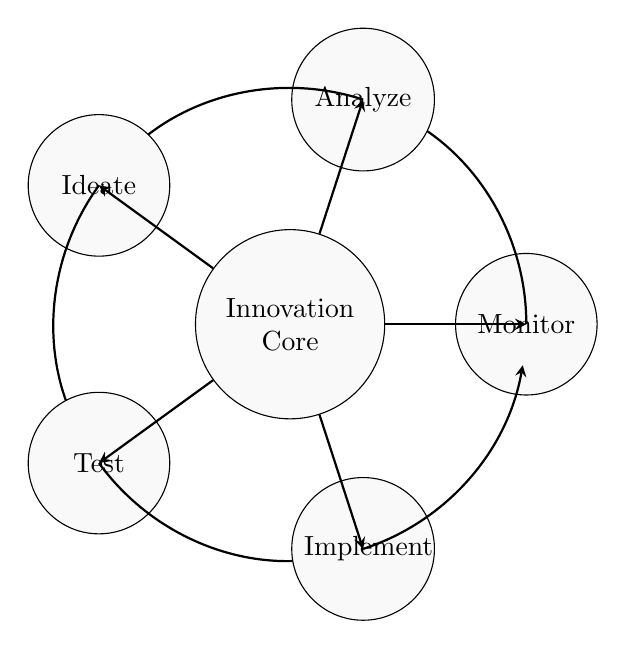
\begin{tikzpicture}[
        node distance=3cm,
        core/.style={draw, circle, text width=2cm, align=center, fill=gray!5},
        phase/.style={draw, circle, text width=1.5cm, align=center, fill=gray!5},
        arrow/.style={-stealth, thick}
    ]
        % Innovation cycle with improved styling
        \node[core] (core) at (0,0) {Innovation\\Core};
        \foreach \angle/\label in {
            0/Monitor,
            72/Analyze,
            144/Ideate,
            216/Test,
            288/Implement
        } {
            \node[phase] at (\angle:3) {\label};
            \draw[arrow] (core) -- (\angle:3);
            \draw[arrow] (\angle:3) arc (\angle:\angle+62:3);
        }
    \end{tikzpicture}
    \caption{Continuous Innovation Cycle}
    \label{fig:innovation-cycle}
\end{figure}

\subsection{Adaptation Matrix}
\begin{center}
\begin{tabularx}{\textwidth}{>{\raggedright\arraybackslash}X >{\centering\arraybackslash}X >{\centering\arraybackslash}X >{\raggedright\arraybackslash}X}
    \toprule
    \textbf{Change Driver} & \textbf{Impact} & \textbf{Timeline} & \textbf{Response Strategy} \\
    \midrule
    Technology & High & Short-term & Digital transformation \\
    Market & Medium & Medium-term & Product evolution \\
    Regulation & High & Long-term & Compliance adaptation \\
    Competition & Medium & Ongoing & Innovation focus \\
    \bottomrule
\end{tabularx}
\end{center}

\section{Emerging Market Trends}

\subsection{Trend Analysis Framework}
\begin{tcolorbox}[colback=white,colframe=primarydark,title=\textbf{Trend Categories}]
\begin{itemize}
    \item Technology Evolution
    \item Consumer Behavior
    \item Regulatory Environment
    \item Market Structure
    \item Competition Dynamics
\end{itemize}
\end{tcolorbox}

\FloatBarrier
\section{Regional Future Outlook}

% UK Region
\begin{regionalbox}{United Kingdom}
\textbf{Financial Services Evolution}
\begin{itemize}
    \item Digital banking transformation
    \item Open banking adoption
    \item RegTech integration
    \item Cross-border innovation
\end{itemize}
\end{regionalbox}

\subsection{UK FinTech Future State}
\begin{figure}[htbp]
    \centering
    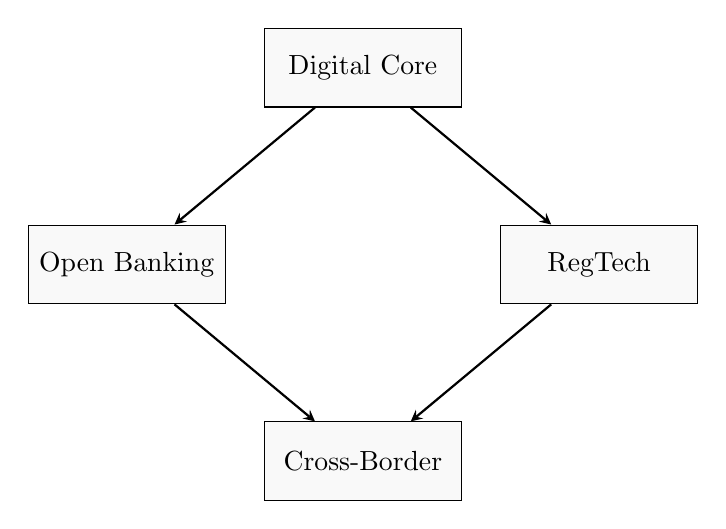
\begin{tikzpicture}[
        node distance=2.5cm,
        box/.style={draw, minimum width=2.5cm, minimum height=1cm, align=center, fill=gray!5},
        arrow/.style={-stealth, thick}
    ]
        % Future state visualization with improved layout
        \node[box] (digital) at (0,0) {Digital Core};
        \node[box] (open) at (-3,-2.5) {Open Banking};
        \node[box] (reg) at (3,-2.5) {RegTech};
        \node[box] (cross) at (0,-5) {Cross-Border};

        % Connect components with styled arrows
        \draw[arrow] (digital) -- (open);
        \draw[arrow] (digital) -- (reg);
        \draw[arrow] (open) -- (cross);
        \draw[arrow] (reg) -- (cross);
    \end{tikzpicture}
    \caption{Future Financial Services Architecture}
    \label{fig:future-fintech}
\end{figure}

% US Region
\begin{regionalbox}{United States}
\textbf{Tech Sector Trends}
\begin{itemize}
    \item AI/ML integration
    \item Cloud native architecture
    \item Edge computing
    \item Blockchain adoption
\end{itemize}
\end{regionalbox}

\subsection{US Tech Evolution Path}
\begin{center}
\begin{tabularx}{\textwidth}{>{\raggedright\arraybackslash}X >{\centering\arraybackslash}X >{\centering\arraybackslash}X}
    \toprule
    \textbf{Technology} & \textbf{Adoption Phase} & \textbf{Impact Level} \\
    \midrule
    AI/ML & Early Majority & High \\
    Cloud Native & Mainstream & Very High \\
    Blockchain & Early Adopters & Medium \\
    \bottomrule
\end{tabularx}
\end{center}

% UAE Region
\begin{regionalbox}{UAE}
\textbf{Trade Pattern Shifts}
\begin{itemize}
    \item Digital trade platforms
    \item Smart logistics
    \item Sustainable practices
    \item Supply chain innovation
\end{itemize}

\subsection{UAE Future Trade Framework}
\begin{tcolorbox}[colback=white,colframe=primary,title=\textbf{Future Trade Components}]
\begin{enumerate}
    \item Digital transformation
    \item Sustainable operations
    \item Smart logistics
    \item Platform integration
    \item Automated compliance
\end{enumerate}
\end{tcolorbox}
\end{regionalbox}

% Canada Region
\begin{regionalbox}{Canada}
\textbf{Sector Development}
\begin{itemize}
    \item Smart agriculture
    \item Clean technology
    \item Digital education
    \item Sustainable practices
\end{itemize}
\end{regionalbox}

\subsection{Canadian Innovation Roadmap}
\begin{center}
\begin{tabularx}{\textwidth}{>{\raggedright\arraybackslash}X >{\raggedright\arraybackslash}X >{\centering\arraybackslash}X}
    \toprule
    \textbf{Sector} & \textbf{Innovation Focus} & \textbf{Timeline} \\
    \midrule
    Agriculture & Smart farming & 2-3 years \\
    CleanTech & Renewable energy & 3-5 years \\
    Education & Digital learning & 1-2 years \\
    \bottomrule
\end{tabularx}
\end{center}

\FloatBarrier
\section{Sustainability Considerations}

\subsection{Sustainability Framework}
\begin{figure}[htbp]
    \centering
    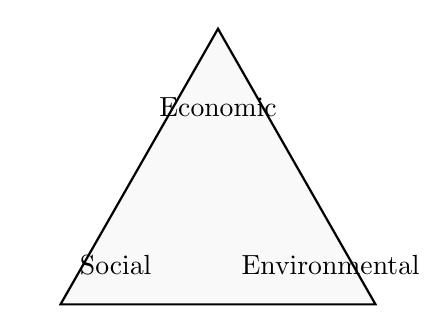
\begin{tikzpicture}[
        node/.style={text width=2cm, align=center}
    ]
        % Sustainability triangle with improved styling
        \path[fill=gray!5] (0,0) -- (4,0) -- (2,3.5) -- cycle;
        \draw[thick] (0,0) -- (4,0) -- (2,3.5) -- cycle;

        \node[node] at (2,2.5) {Economic};
        \node[node] at (0.7,0.5) {Social};
        \node[node] at (3.3,0.5) {Environmental};
    \end{tikzpicture}
    \caption{Triple Bottom Line Approach}
    \label{fig:sustainability}
\end{figure}

\section{Exit Strategy Planning}

\begin{tcolorbox}[colback=white,colframe=primarydark,title=\textbf{Exit Options Analysis}]
\begin{itemize}
    \item Strategic Sale
    \item Initial Public Offering
    \item Management Buyout
    \item Succession Planning
\end{itemize}
\end{tcolorbox}

\begin{communitybox}
Stay updated on future trends through the Africa Growth Circle:
\begin{itemize}
    \item Trend analysis reports
    \item Innovation workshops
    \item Expert webinars
    \item Market forecasts
    \item Sustainability guides
\end{itemize}
Visit circle.counseal.com for ongoing support.
\end{communitybox}

\begin{workshopbox}
\textbf{Chapter 10 Future Planning Workshop}

1. Innovation Strategy
\begin{itemize}
    \item Key trends to monitor: \_\_\_\_\_\_\_\_\_
    \item Innovation priorities: \_\_\_\_\_\_\_\_\_
    \item Resource allocation: \_\_\_\_\_\_\_\_\_
\end{itemize}

2. Sustainability Planning
\begin{itemize}
    \item Environmental impact: \_\_\_\_\_\_\_\_\_
    \item Social responsibility: \_\_\_\_\_\_\_\_\_
    \item Economic sustainability: \_\_\_\_\_\_\_\_\_
\end{itemize}

3. Long-term Vision
\begin{itemize}
    \item 5-year goals: \_\_\_\_\_\_\_\_\_
    \item Exit strategy: \_\_\_\_\_\_\_\_\_
    \item Legacy planning: \_\_\_\_\_\_\_\_\_
\end{itemize}

Access future planning tools and resources on the Africa Growth Circle platform.
\end{workshopbox}

\begin{importantbox}
Congratulations on completing this comprehensive guide! Remember to stay connected with the Africa Growth Circle community for ongoing support and updates as you build your success in the Nigerian market.
\end{importantbox}